\documentclass{report}
\usepackage[showframe=false]{geometry}
\usepackage{titlesec}
\usepackage{amsmath}
\usepackage{graphicx}
\usepackage{tikz,pgfplots}

\usepgfplotslibrary{fillbetween}
\usepgfplotslibrary{groupplots}
\usetikzlibrary{arrows,shapes.multipart,calc}

\pagenumbering{gobble}

\geometry{tmargin=60pt,bmargin=90pt,lmargin=90pt,
rmargin=90pt}

\titleformat{\chapter}{\normalfont\huge}{\thechapter.}{20pt}{\huge}
\titlespacing*{\chapter} {0pt}{0pt}{10pt}

\definecolor{cadmiumgreen}{rgb}{0.0, 0.42, 0.24}

\begin{document}

\chapter{Question 1}

Consider  one auto  company that  receives  parts from  three suppliers;  assume  
50\% of  the parts from  supplier  1,  30\% from  supplier  2,  and 20\% from  supplier  3.  
The quality of  the parts could be  summarized  in  the following table based on  
historically  data.

\begin{center}
  \begin{tabular}{ | c | c | c | } 
    \hline
      & Percentage Good Parts & Percentage Bad parts \\ 
    \hline
    Supplier 1 & 98 & 2 \\ 
    \hline
    Supplier 2 & 95 & 5 \\ 
    \hline
    Supplier 3 & 92 & 8 \\ 
    \hline
  \end{tabular}
\end{center}

Question: A bad part  broke one of  the machines  (observed), what  is  the 
probability the part  came  from  supplier  1?

\hspace{1cm}

\textbf{ANSWER:} \\

Let $A_1$ denote Supplier 1, $A_2$ denote Supplier 2, and $A_3$ denote Supplier 3

\begin{equation} \label{eq3}
  \begin{split}
    P(A_1) & = 0.50 \\
    P(A_2) & = 0.30 \\
    P(A_3) & = 0.20 \\
  \end{split}
\end{equation}

Let G denote that a part is good and B denote that a part is bad. \\

\begin{equation} \label{eq3}
  \begin{split}
    P(G|A_1) & = 0.98 \\
    P(G|A_2) & = 0.95 \\
    P(G|A_3) & = 0.92 \\
  \end{split}
\end{equation}

\begin{equation} \label{eq3}
  \begin{split}
    P(B|A_1) & = 0.02 \\
    P(B|A_2) & = 0.05 \\
    P(B|A_3) & = 0.08 \\
  \end{split}
\end{equation}

\break

Here is the Probability Tree for Three-Suppliers

\hspace{1cm}

% Set the overall layout of the tree
\tikzstyle{level 1}=[level distance=3.5cm, sibling distance=3.5cm]
\tikzstyle{level 2}=[level distance=3.5cm, sibling distance=2cm]

% Define styles for bags and leafs
\tikzstyle{bag} = [circle, minimum width=3pt, fill, inner sep=0pt]
\tikzstyle{end} = [circle, minimum width=3pt, fill, inner sep=0pt]

% The sloped option gives rotated edge labels. Personally
% I find sloped labels a bit difficult to read. Remove the sloped options
% to get horizontal labels. 
\begin{tikzpicture}[grow=right, sloped]
  \node[bag] {$\circ$}
  child {
    node[bag] {$\circ$}
    child {
      node[end, label=right:
      {$P(A_3\cap B)=P(A_3)P(B|A_3)=0.016$}] {}
      edge from parent
      node[above] {$P(B|A_3)$}
    node[below]  {\textcolor{red}{$0.08$}}
    }
    child {
      node[end, label=right:
      {$P(A_3\cap G)=P(A_3)P(G|A_3)=0.184$}] {}
      edge from parent
      node[above] {$P(G|A_3)$}
      node[below]  {\textcolor{cadmiumgreen}{$0.92$}}
    }
    edge from parent 
    node[above] {$P(A_3)$}
    node[below]  {\textcolor{blue}{$0.20$}}
  } child {
    node[bag] {$\circ$}
    child {
      node[end, label=right:
      {$P(A_2\cap B)=P(A_2)P(B|A_2)=0.015$}] {}
      edge from parent
      node[above] {$P(B|A_2)$}
      node[below]  {\textcolor{red}{$0.05$}}
    }
    child {
      node[end, label=right:
      {$P(A_2\cap G)=P(A_2)P(G|A_2)=0.285$}] {}
      edge from parent
      node[above] {$P(G|A_2)$}
      node[below]  {\textcolor{cadmiumgreen}{$0.95$}}
    }
    edge from parent         
    node[above] {$P(A_2)$}
    node[below]  {\textcolor{blue}{$0.30$}}
  } child {
    node[bag] {$\circ$}
    child {
      node[end, label=right:
      {$P(A_1\cap B)=P(A_1)P(B|A_1)=0.010$}] {}
      edge from parent
      node[above] {$P(B|A_1)$}
      node[below]  {\textcolor{red}{$0.02$}}
    }
    child {
      node[end, label=right:
      {$P(A_1\cap G)=P(A_1)P(G|A_1)=0.490$}] {}
      edge from parent
      node[above] {$P(G|A_1)$}
      node[below]  {\textcolor{cadmiumgreen}{$0.98$}}
    }
    edge from parent         
    node[above] {$P(A_1)$}
    node[below]  {\textcolor{blue}{$0.50$}}
  };
\end{tikzpicture}

\hspace{1cm}

Law of Conditional Probability gives us the following equation

\begin{equation} \label{eq3}
  P(A_1|B) = \frac{P(A_1\cap B)}{P(B)}
\end{equation}

We know from are probability tree that

\begin{equation} \label{eq3}
P(A_1\cap B)=P(A_1)P(B|A_1)=0.010
\end{equation}

We also know that

\begin{equation} \label{eq3}
  P(B) = P(A_1\cap B) + P(A_2\cap B) + P(A_3\cap B) = P(A_1)P(B|A_1) + P(A_2)P(B|A_2) + P(A_3)P(B|A_3)
\end{equation}

Combining are equations togther we obtain Bayes' Theorem

\begin{equation}
  \begin{split}
    & 1 \leq k \leq n \\
    P(B_k|A) & = \frac{P(A|B_k)P(B_k)}{\sum_{i=1}^{n}P(A|B_i)P(B_i)}
  \end{split}
\end{equation}

\begin{equation}
  \begin{split}
    P(A_1|B) & = \frac{P(A_1)P(B|A_1)}{P(A_1)P(B|A_1)+P(A_2)P(B|A_2)+P(A_3)P(B|A_3)} \\
    P(A_2|B) & = \frac{P(A_2)P(B|A_2)}{P(A_1)P(B|A_1)+P(A_2)P(B|A_2)+P(A_3)P(B|A_3)} \\
    P(A_3|B) & = \frac{P(A_3)P(B|A_3)}{P(A_1)P(B|A_1)+P(A_2)P(B|A_2)+P(A_3)P(B|A_3)} \\
  \end{split}
\end{equation}

\break

Now all we have to do is plug in the numbers and solve the equations

\begin{equation}
  \begin{split}
  P(A_1|B) & = \frac{(0.50)(0.02)}{(0.50)(0.02)+(0.30)(0.05) +(0.20)(0.08)} = \frac{0.010}{0.041} = 0.2439024390 \\
  P(A_2|B) & = \frac{(0.30)(0.05)}{(0.50)(0.02)+(0.30)(0.05) +(0.20)(0.08)} = \frac{0.015}{0.041} = 0.3658536585 \\
  P(A_3|B) & = \frac{(0.20)(0.08)}{(0.50)(0.02)+(0.30)(0.05) +(0.20)(0.08)} = \frac{0.016}{0.041} = 0.3902439024 \\
  \end{split}
\end{equation}

Therefore the probability the part came from supplier 1: 0.243902439

\chapter{Question 2}

For the play  tennis  data  set shown below:

\begin{tabular}{ |c||c c c c | c | }
  \hline
  Day & Outlook & Temperature & Humidity & Wind & PlayTennis \\
  \hline
  D1  & Sunny                     & Hot                   & High                    & Weak                    & No                   \\
  D2  & Sunny                     & Hot                   & High                    & Strong                  & No                   \\
  D3  & \textcolor{red}{Overcast} & \textcolor{red}{Hot}  & \textcolor{red}{High}   & \textcolor{red}{Weak}   & \textcolor{red}{Yes} \\
  D4  & \textcolor{red}{Rain}     & \textcolor{red}{Mild} & \textcolor{red}{High}   & \textcolor{red}{Weak}   & \textcolor{red}{Yes} \\
  D5  & \textcolor{red}{Rain}     & \textcolor{red}{Cool} & \textcolor{red}{Normal} & \textcolor{red}{Weak}   & \textcolor{red}{Yes} \\
  D6  & Rain                      & Cool                  & Normal                  & Strong                  & No                   \\
  D7  & \textcolor{red}{Overcast} & \textcolor{red}{Cool} & \textcolor{red}{Normal} & \textcolor{red}{Strong} & \textcolor{red}{Yes} \\
  D8  & Sunny                     & Mild                  & High                    & Weak                    & No                   \\
  D9  & \textcolor{red}{Sunny}    & \textcolor{red}{Cool} & \textcolor{red}{Normal} & \textcolor{red}{Weak}   & \textcolor{red}{Yes} \\
  D10 & \textcolor{red}{Rain}     & \textcolor{red}{Mild} & \textcolor{red}{Normal} & \textcolor{red}{Weak}   & \textcolor{red}{Yes} \\
  D11 & \textcolor{red}{Sunny}    & \textcolor{red}{Mild} & \textcolor{red}{Normal} & \textcolor{red}{Strong} & \textcolor{red}{Yes} \\
  D12 & \textcolor{red}{Overcast} & \textcolor{red}{Mild} & \textcolor{red}{High}   & \textcolor{red}{Strong} & \textcolor{red}{Yes} \\
  D13 & \textcolor{red}{Overcast} & \textcolor{red}{Hot}  & \textcolor{red}{Normal} & \textcolor{red}{Weak}   & \textcolor{red}{Yes} \\
  D14 & Rain                      & Mild                  & High                    & Strong                  & No                   \\
  \hline
\end{tabular}

\section{Part 1}

Please use	Naïve	Bayes	to	help	make	decision	on	playing	tennis	or	not	when
Outlook	is	rain,	Temperature	is	mild,	Humidity	is	normal and	Wind	is	weak.

\hspace{1cm}

\textbf{ANSWER:} \\

\begin{tabular}{ |c|c|c|c| }
  \hline
  \textbf{OUTLOOK} & Play=Yes & Play=No & Total \\
  \hline
  Sunny            & 2/9      & 3/5     & 5/14  \\
  \hline
  Overcast         & 4/9      & 0/5     & 4/14  \\
  \hline
  Rain             & 3/9      & 2/5     & 5/14  \\
  \hline
\end{tabular}

\vspace*{1 cm}

\begin{tabular}{ |c|c|c|c| }
  \hline
  \textbf{TEMPERATURE} & Play=Yes & Play=No & Total \\
  \hline
  Hot                  & 2/9      & 2/5     & 4/14  \\
  \hline
  Mild                 & 4/9      & 2/5     & 6/14  \\
  \hline
  Cool                 & 3/9      & 1/5     & 4/14  \\
  \hline
\end{tabular}

\vspace*{1 cm}

\begin{tabular}{ |c|c|c|c| }
  \hline
  \textbf{HUMIDITY} & Play=Yes & Play=No & Total \\
  \hline
  High              & 3/9      & 4/5     & 7/14  \\
  \hline
  Normal            & 6/9      & 1/5     & 7/14  \\
  \hline
\end{tabular}

\vspace*{1 cm}

\begin{tabular}{ |c|c|c|c| }
  \hline
  \textbf{WIND} & Play=Yes & Play=No & Total \\
  \hline
  Strong        & 3/9      & 3/5     & 6/14  \\
  \hline
  Weak          & 6/9      & 2/5     & 8/14  \\
  \hline
\end{tabular}

\begin{equation*}
  \begin{split}
    P(Play=Yes) & = 9/14 \\
    P(Play=No)  & = 5/14 \\
  \end{split}
\end{equation*}

Let x' denote the conditions of playing tennis or not

$x' = (Outlook=Rain, Temperature=Mild, Humidity=Normal, Wind=Weak)$

The probability that tennis is played lookup table

\begin{equation*}
  \begin{split}
    P(Outlook=Rain|Play=Yes)     & = 3/9 \\
    P(Temperature=Mild|Play=Yes) & = 4/9 \\
    P(Humidity=Normal|Play=Yes)  & = 6/9 \\
    P(Wind=Weak|Play=Yes)        & = 6/9 \\
  \end{split}
\end{equation*}

\begin{equation*}
  \begin{split}
    P(Outlook=Rain|Play=No)     & = 2/5 \\
    P(Temperature=Mild|Play=No) & = 2/5 \\
    P(Humidity=Normal|Play=No)  & = 1/5 \\
    P(Wind=Weak|Play=No)        & = 2/5 \\
  \end{split}
\end{equation*}

Now we can construnct the following equation

\begin{equation*}
  \begin{split}
    P(Play=Yes|x') & = P(x'|Play=Yes)P(Play=Yes) \\
    & = [P(Rain|Yes)P(Mild|Yes)P(Normal|Yes)P(Weak|Yes)]P(Play=Yes) \\
    & = (3/9 * 4/9 * 6/9 * 6/9)(9/14) \\
    & = 0.0423280423 \\
  \end{split}
\end{equation*}

\begin{equation*}
  \begin{split}
    P(Play=No|x')  & = P(x'|Play=No)P(Play=No) \\
    & = [P(Rain|No)P(Mild|No)P(Normal|No)P(Weak|No)]P(Play=No) \\
    & = (2/5 * 2/5 * 1/5 * 2/5)(5/14) \\
    & = 0.0045714286 \\
  \end{split}
\end{equation*}

Given The Fact that $P(Play=Yes|x') > P(Play=No|x')$ we would label x' to be Yes

\section{Part 2}

	The	humidity	value	could	be	continuous	practically.	In	the	above	data	set,	if
the	humidity	value	is	as	follows per	original	data	set	order:
\begin{equation*}
  \begin{split}
    Yes: & 65.7,	20.7,	5.1,	6.9,	4.8,	6.9,	8.7,	10.4,	15.3, \\
    No:	& 58.1,	66.4,	6.5,	10.5,	12.8 \\
  \end{split}
\end{equation*}
Please	use	Naïve	Bayes	to	help	make	decision	on	playing	tennis	or	not	when	the
Outlook	is	Overcast,	Temperature	is	mild,	Humidity	is	8.8,	and	Wind	is	weak.

\chapter{Question 3}

We  have  a training  dataset as  follows:

\vspace*{0.5 cm}

\begin{tabular}{ |c|c|c| }
  \hline
  Feature 1 & Feature 2 & Label \\
  \hline
  6         & 6         & L1    \\
  \hline
  6         & 4         & L1    \\
  \hline
  2         & 3         & L2    \\
  \hline
  1         & 4         & L2    \\
  \hline
\end{tabular}

\vspace*{0.5 cm}

Using K-NN  algorithm to  determine the label for a new data  record  (3, 6). The 
similarity  measure is  assumed to  be  Euclidean distance.

\vspace*{0.5 cm}

\begin{tikzpicture}
  \begin{axis}[%
      scatter/classes={%
        L1={color=blue},
        L2={color=red},
        L3={color=black}
    }]
    \addplot[scatter,only marks,%
    scatter src=explicit symbolic]%
    table[meta=label] {
      x y label
      6 6 L1
      6 4 L1
      2 3 L2
      1 4 L2
      3 6 L3
    };
  \end{axis}
\end{tikzpicture}

Using Euclidean Distance we can calculate the distances between the two points

\begin{equation*}
  d(x_i, x_j) = \sqrt{\sum_{r=1}^{n}(f_r(x_i)-f_r(x_j))^2} 
\end{equation*}

Using Euclidean Distance we get the following results

\begin{equation*}
  \begin{split}
    (6, 6, L1): \sqrt{(6-3)^2 + (6-6)^2} & = \sqrt{9} = 3 \\
    (6, 4, L1): \sqrt{(6-3)^2 + (4-6)^2} & = \sqrt{13} = 3.605551275 \\
    (2, 3, L2): \sqrt{(2-3)^2 + (3-6)^2} & = \sqrt{10} = 3.16227766 \\
    (1, 4, L2): \sqrt{(1-3)^2 + (4-6)^2} & = \sqrt{8} = 2.828427125 \\
  \end{split}
\end{equation*}

Using K=1 we can see that the new data record of (3, 6) would be classified as L2

Using K=2 the new data record is split between L1 and L2

Using K=3 we can see that the new data record of (3, 6) would be classified as L2

Using K=4 the new data record is split between L1 and L2

\chapter{Question 4}

Given the following 12  data  points x=(x1, x2) in  the training  data  set.

\begin{equation*}
  (1, 3), (2, 5), (3, 15),  (4, 8), (4, 19),  (5, 6), (6, 13), \\
  (8, 6), (10,  15),  (12,  7), (15,  4), (17,  18)
\end{equation*}

\section{Part 1}
If  we  know  the value range of  features  x1, x2  is  in  [0, 20],  please  build the 
quadtree. 

\pgfmathsetmacro{\wdbox}{.02\textwidth}
\tikzset{
  >= stealth, 
  every picture/.style={ultra thick},
  every node/.style={anchor=north},
  simple/.style={draw,minimum size=3*\wdbox,scale=.8},
  array/.style={%
              draw,scale=.8, 
              inner sep=\wdbox, 
              rounded corners,
              rectangle, 
              rectangle split, 
              rectangle split parts=4,
              rectangle split ignore empty parts=false, 
              rectangle split horizontal,
              append after command={%
              \pgfextra{\let\mainnode=\tikzlastnode} 
              coordinate (c1 \mainnode) at ($(\mainnode.west)!.5!(\mainnode.one split)$)
              coordinate (c2 \mainnode) at ($(\mainnode.one split)!.5!(\mainnode.two split)$)
              coordinate (c3 \mainnode) at ($(\mainnode.two split)!.5!(\mainnode.three split)$)
              coordinate (c4 \mainnode) at ($(\mainnode.three split)!.5!(\mainnode.east)$)                
                    }
                  }
                }

  \begin{tikzpicture}[x=.035\textwidth,y=.035\textwidth]
       \node[simple] (1) {};
       \draw[->] (1.center) -- +( 0,-2) node[array]  (2) {};
       \draw[->] (c1 2)     -- +(-3,-2) node[simple] (3) {};
       \draw[->] (c2 2)     -- +(-1,-2) node[simple] (4) {};  
       \draw[->] (c3 2)     -- +( 0,-2) node         (5) {$\emptyset$};
       \draw[->] (c4 2)     -- +(+3,-2) node[simple] (6) {};
       \draw[->] (3.center) -- +( 0,-2) node[array]  (7) {};         
       \draw[->] (4.center) -- +( 0,-2) node         (8) {$\emptyset$};       
       \draw[->] (c1 7)     -- +(-3,-2) node[simple] (9) {};
  \end{tikzpicture}

  \pgfkeys{
    /prepare label/.style={
      /print label/\detokenize{#1}/.code={\ttfamily\detokenize{#1}}
    },
    /prepare label/.list={a,b,c,d,e,f,g,h,i,j,k,l}
  }

  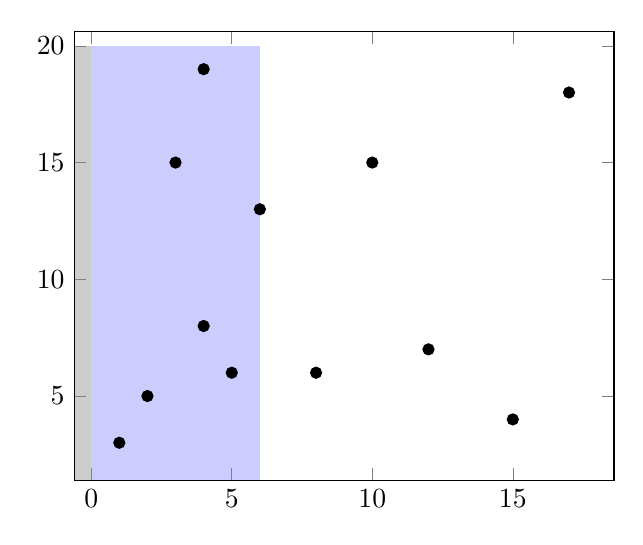
\begin{tikzpicture}
    \begin{axis}[%
        axis background/.style={%
          preaction={
            path picture={
              \fill [black!20] (axis cs:-6,0) rectangle (axis cs:0,20);
              \fill [blue!20] (axis cs:6,0) rectangle (axis cs:0,20);
            }
          }
        }
      ]
      \addplot[
        mark=*,
        only marks,
        point meta=explicit symbolic,
        nodes near coords={
          \pgfkeys{/print label/\pgfplotspointmeta/.try}
        }
      ]
      table[header=false,meta index=0,x index=1,y index=2]{
        a   1  3
        b   2  5
        c   3 15
        d   4  8
        e   4 19
        f   5  6
        g   6 13
        h   8  6
        i  10 15
        j  12  7
        k  15  4
        l  17 18
      };
    \end{axis}
  \end{tikzpicture}

\section{Part 2}
Using the quadtree  learnt  in  4.1 to  find  the nearest neighbor  of  data  point 
(11,  16).

\end{document}
